%%%%%%%%%%%%%%%%%%%%%%%%%%%%%%%%%%%
%%%%%%%%%%%%%%%%%bardproj_template.tex%%%%%%
%%
%% This is a template for the Bard Project Style.
%%
%% Copy it to a new file with a new name and use it as the basis
%% for your Bard senior project or M.A.T. mathematics research project.
%%
%% Replace everything inside <   > with the appropriate text,
%% and remove the <   >.
%%
%% Put a comment symbol (%) before anything in the template you 
%% do not need.
%%
%% Add as many additional chapters, sections and bibliographic 
%% entries as you need.
%%
%% Read the manual bardproj_man.tex or bardproj_man.pdf 
%% for more details regarding the Bard Project Style.
%%
%% The Bard Project Style file and the manual for this style file
%% can be found at http://math.bard.edu/bloch/bardtex.htm
%%
%% For additional help, or for suggestions or corrections
%% contact Ethan Bloch at bloch@bard.edu
%%
%%%%%%%%%%%%Bard Senior Project Style %%%%%%%%%
%%%%%%%%%%%%%%%%%%%%%%%%%%%%%%%%%%%

\documentclass[11pt, oneside, reqno]{book}
\usepackage{amssymb, amsthm, amsmath, amsfonts}
\usepackage{bardproj}
\usepackage{graphicx} %this used to be graphics, which maybe is wrong
\usepackage{amsrefs}
% Packages added by me:
\usepackage{caption}

%<Your macros, if you have any>



\begin{document}

%For senior projects:
\titlepg{Anamorphic Projections}{Van Mai Nguyen Thi}
    {May}{2015}

%For M.A.T. mathematics research projects, uncomment the following, and remove the above:
%\titlepgmat{<Title of Project>}{<Your Name>}
%    {<Month of Graduation>}{<Year of Graduation>}

\abstr

<Text of abstract>

\tableofcontents

\dedic

<Text of dedication> 

\acknowl

<Text of acknowledgments>

\doublespace


%TODO CH1: Introduction Chapter (bg, definitions)
\chapter{Introduction}
\label{chap:int}

\section{Background}
\label{sec:bac}

An anamorphosis (or anamorphic projection/image) is an image that is intentionally distorted so that the original image can be recovered only when looked at from a certain point of view or using a special device, for example a mirror. Origins of anamorphosis can be traced back to the 16th century art where artists, mathematicians and philosophers, fascinated by the idea of perspective, experimented with the notions of illusion, truth and reality.~\cite{bib:ana_hun} Some of the notable examples of anamorphosis included Jean-Francois Niceron's methods for geometrical construction that generated multiple types of anamorphic transforms which involved both exact and approximate methods.~\cites{bib:ana_hun,bib:per_nic} One of the most famous anamorphic paintings is Hans Holbein's \textit{The Ambassadors} (Figure \ref{fig:hol}), in which the artist embedded an anamorphic image of a skull (Figure \ref{fig:hol_sku}) at the bottom of the painting as a \textit{memento mori}, a recurring motif in many artworks in the Renaissance period.

%\begin{figure}
%\centering
%\begin{minipage}{.46\textwidth}
%	\centering
%	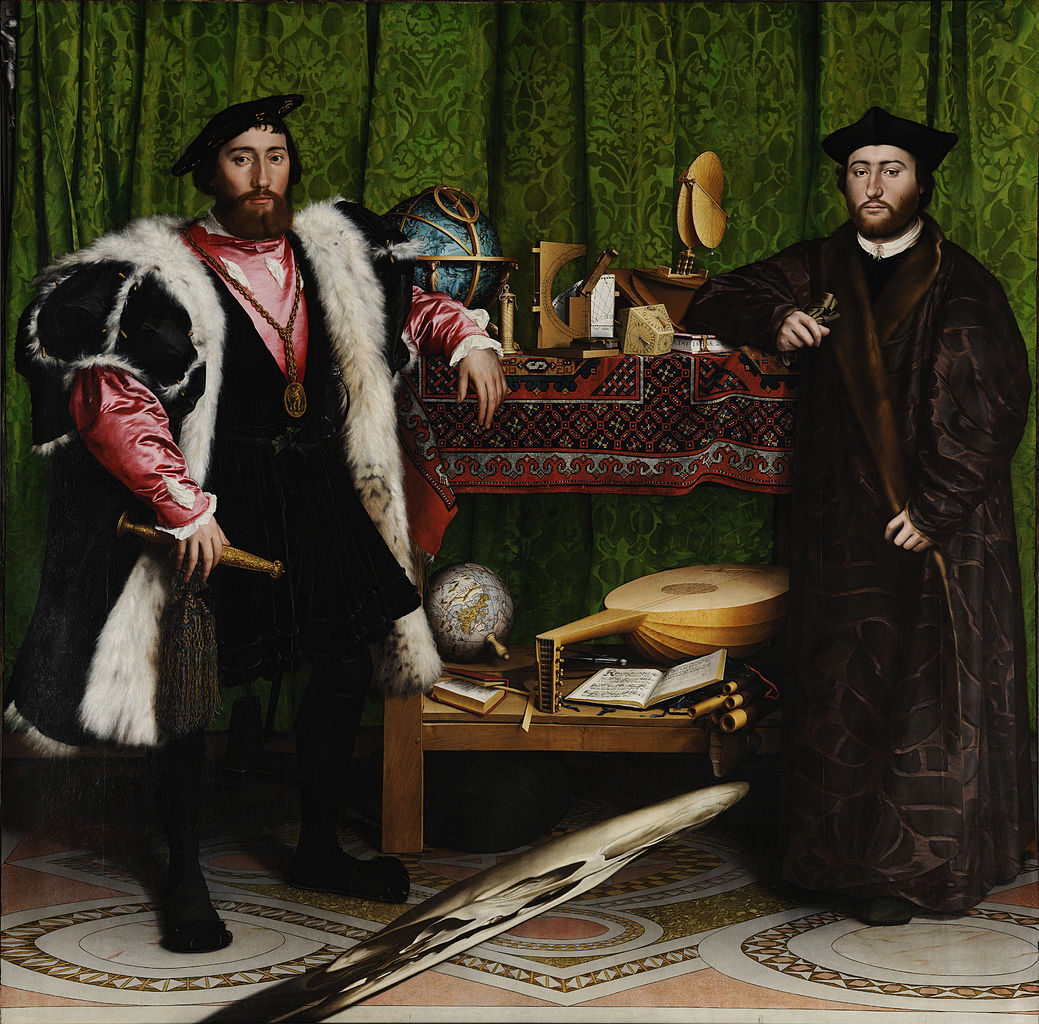
\includegraphics[width=\linewidth]{data/Holbein1}
%	\captionof{figure}{Hans Holbein's \textit{The Ambassadors}, 1533 <Add reference>}%TODO add
%	\label{fig:hol}
%\end{minipage}%
%\qquad\begin{minipage}{.45\textwidth}
%	\centering
% 	\includegraphics[width=.9\linewidth]{data/Holbein_Skull}
%  	\captionof{figure}{Undistorted skull from H. Holbein's \textit{The Ambassadors} <Add reference>} %TODO add reference
%  	\label{fig:hol_sku}
%\end{minipage}
%\end{figure}

\begin{figure}
\centering
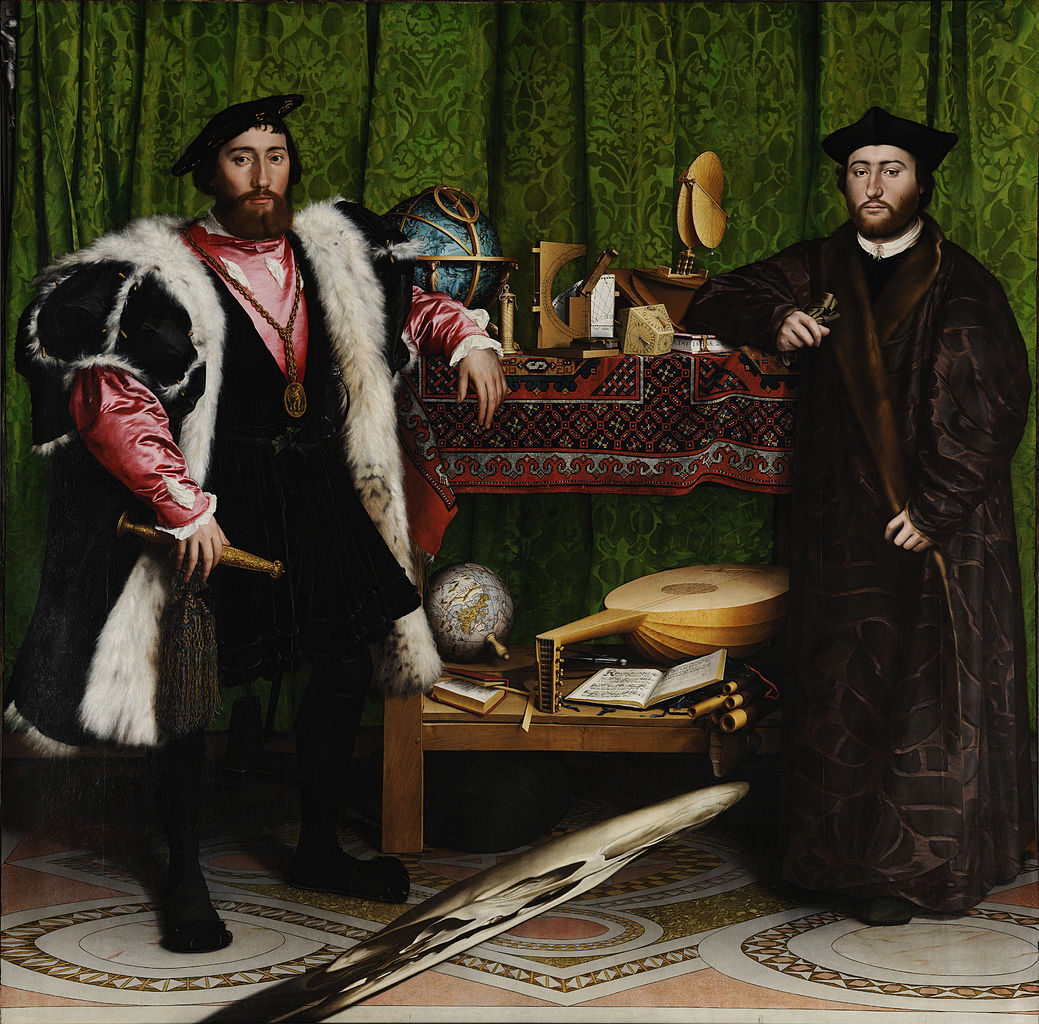
\includegraphics[width=0.6\textwidth]{data/Holbein1}
\caption{Hans Holbein's \textit{The Ambassadors}, 1533 <Add reference>} %TODO add reference
\label{fig:hol}
\end{figure}

\begin{figure}
\centering
\includegraphics[width=0.4\textwidth]{data/Holbein_Skull}
\caption{Undistorted skull from H. Holbein's \textit{The Ambassadors} <Add reference>} %TODO add reference
\label{fig:hol_sku}
\end{figure}

Anamorphosis is still prevalent to this day, and is incorporated in many new forms of art, most noticeably street art. The undying fascination for anamorphosis is manifested in numerous artworks centered around the anamorphic principle and using it to create a unique piece of art.

Beyond the esthetic values, anamorphosis has found its uses in many practical settings, such as road signs that are elongated so that drivers' looking at them from a small angle above the ground can see the signs correctly (Figure \ref{fig:bik}), or inverted ``ambulance" signs that are meant to be reflected correctly in the rear-view mirrors.

However, despite the widespread uses, there is a surprising lack of detailed explanation of the mathematical principles behind anamorphosis, and even with the advanced technology there is hardly any computer software generating the anamorphic projections. The goal of this project is two-fold. First of all, we need to build a comprehensive documentation describing the most common types of anamorphosis. Next, we will apply the acquired knowledge to create a software that will automate the process of generating anamorphic projections.

\begin{figure}[h]
\centering
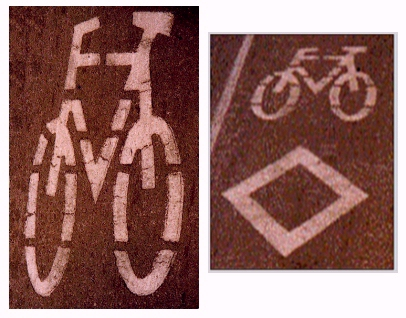
\includegraphics[width=0.6\textwidth]{data/bikes}
\caption{Road sign in the shape of an elongated bike. Left: view from the top; right: view from a driver's perspective.~\cite{bib:ana_hun}}
\label{fig:bik}
\end{figure}



\section{Definitions}
\label{sec:def}

In this section we define some basic concepts and terminology needed to describe anamorphic projections. In particular, we introduce homogeneous representations of geometrical objects used in computer vision to facilitate computing geometrical transformations.

\subsection{Basic geometry}
In mathematics, geometric elements in a coordinate system are most commonly represented in Cartesian coordinates. 

\begin{definition}[Cartesian point]  
\label{def:cpoint}
Let $P$ be a point in $n$ dimensions positioned in a coordinate system. The $n$-tuple $(x_1, x_2, ..., x_n)$ is its representation in Cartesian coordinates if $x_i$ is the distance from point $P$ to the origin along the $i^{th}$ axis for all $i \le n$.
\end{definition}

\begin{definition}[Cartesian line]  
\label{def:cline}
<def line> %TODO
\end{definition}



\subsection{Homogeneous representation}
Homogeneous coordinates were first defined by August Ferdinand M\"{o}bius as <... why?>. ~\cite{history} They are widely used in computer vision, as they offer a convenient way to perform projective transformations.

\begin{definition}[Homogeneous point]  
\label{def:hpoint}
Let $P$ be a point in $n$ dimensions, and $(x_1, x_2, ..., x_n)$ be its representation in Cartesian coordinates. The homogeneous representation of $P$ is any $(n+1)$-tuple $(x_1\omega, x_2\omega, ..., x_n\omega, \omega)$, where $\omega$ is called the homogeneous coordinate. 
\end{definition}

A Cartesian point can be easily written as a homogeneous point by appending $\omega=1$ as the $(n+1)^{th}$ coordinate. A homogeneous point can be converted to Cartesian coordinates by dividing each of its coordinates by $\omega$, and removing the homogenous coordinate.

\begin{lemma}
\label{lem:multHpoint}
When a homogeneous point is multiplied by a scalar, it is the same point.
\end{lemma}
<prove this lemma?> Should this be a lemma or just a "narrative"?

\begin{example}
\label{ex:cartHomo}
Let $P_1$ be a point in three dimensions with Cartesian coordinates $(x,y,z)$. A possible homogeneous representation of $P_1$ is $(x,y,z,1)$, or more generally $(x\omega, y\omega, z\omega, \omega)$ for any $\omega$ (<$\omega \ge 0$???>).
Let $P_2$ be another point in three dimensions with homogeneous representation $(x,y,z,\omega)$. $P_2$ can be represented in Cartesian coordinates as $\left(\frac{x}{\omega}, \frac{y}{\omega}, \frac{z}{\omega}\right)$.
\end{example}

\begin{definition}[Homogeneous line in 2D] 
\label{def:hline}
Let $l$ be a straight line in two dimensions defined by the equation $ax+by+c = 0$. Then $(a,b,c)$ is the homogeneous representation of $l$.
\end{definition}

\begin{lemma}[Intersection of lines in 2D]
\label{lem:intersect}
A point $P$ is the intersection of two-dimensional lines $l_1$ and $l_2$ if and only if $P$ is the dot product of $l_1$ and $l_2$ in homogeneous coordinates.
\end{lemma}
\begin{proof}
Let $l_1$ and $l_2$ be two-dimensional lines represented as $(a_1,b_1,c_1)$ and $(a_2,b_2,c_2)$ respectively. 
\end{proof}


\begin{definition}[Degrees of freedom]  
\label{def:degrees}
Let $P$ be a point in $n$ dimensions, and $(x_1, x_2, ..., x_n)$ be its representation in Cartesian coordinates. The homogeneous representation of $P$ is any $(n+1)$-tuple $(x_1\omega, x_2\omega, ..., x_n\omega, \omega)$, where $\omega$ is called the homogeneous coordinate. 
\end{definition}


% END of Homogeneous representation subsection




\subsection{2D Transformations}

\begin{definition}[Translation]  
\label{def:translation}

\end{definition}

\begin{definition}[Scaling]  
\label{def:scaling}

\end{definition}

\begin{definition}[Rotation]  
\label{def:rotation}

\end{definition}

\begin{definition}[Warping]  
\label{def:warp}

\end{definition}

\begin{definition}[Forward Warping]  
\label{def:forwarp}

\end{definition}

\begin{definition}[Backward Warping]  
\label{def:backwarp}

\end{definition}

\begin{definition}[Homography]  
\label{def:homography}
A homography or projective transformation is a transformation of a two-dimensional image $I$ to another two-dimensional image $I'$ (called the anamorphic image), such that all lines in $I$ are preserved in $I'$, or more rigorously. The homography can be represented as a $3 \times 3$ matrix $H$. The anamorphic image is obtained by applying $H$ to every point in the original image to obtain the corresponding point in the anamorphic image:
\[ p'=Hp \text{, for all points } x\in I. \] %TODO looks like same x', different x...
Line preservation means that the points $p_1, p_2, p_3 \in I$ lie on the same line if and only if $Hp_1, Hp_2, Hp_3$ are on the same line.
\end{definition}


% END of 2D Transformations subsection




\subsection{Types of anamorphosis}

\begin{definition}[Perspective anamorphosis]
\label{def:perspective}
Let $S$ be a surface and $V$ be a viewer at some distance $d$ looking directly at the surface $S$ at some angle $\theta$. Let $I$ be some two-dimensional image. $I’$ is an anamorphic projection of $I$ on the surface $S$ for the viewer $V$ if the resulting image that $V$ sees when looking at $S'$ is $S$.
\end{definition}

\begin{definition}[Planar anamorphosis]
\label{def:pla}
This is my definition of planar anamorphosis. 
\end{definition}


% END of Perspective anam. subsection

% END of Definitions section

%%% END of Introduction Chapter






%TODO CH2: Anamorph (Theory/Math) Chapter
\chapter{Anamorphic Projections}
\label{chap:ana}


\section{Planes}
\label{sec:pla}

The relation between the anamorphic (distorted) image on a plane and the correct image that the viewer observes can be described using a 3D homography matrix.

\section{Multiple Planes}
\label{sec:mul}

<Text>

\section{Cylinders}
\label{sec:cyl}

<Text>

\section{Cones}
\label{sec:con}

<Text>

\section{Mirrors}
\label{sec:mir}

<Text>

%\begin{figure}[ht]
%\centering
%\includegraphics{<Path+filename>}
%\caption{<Caption>}
%\label{<Figure Label>}
%\end{figure}

%%% END of Anamorph (Theory/Math) Chapter



%TODO CH3: Methods Chapter
\chapter{Methods}
\label{chap:met}


Def. Least squares

Ransac

Corner detection


\section{<Title of First Section>}
\label{sec:A1}

<Text>

\section{<Title of Second Section>}
\label{sec:AB}

<Text>

%\begin{figure}[ht]
%\centering
%\includegraphics{<Path+filename>}
%\caption{<Caption>}
%\label{<Figure Label>}
%\end{figure}


%%% END of writing





\listoffigures



\singlespace

%TODO Bibliography
\begin{bibdiv}
\begin{biblist}[\normalsize]

\addcontentsline{toc}{chapter}{Bibliography}
\markboth{Bibliography}{Bibliography}

%\bibliography{bibtex}

\bib{bib:ana_hun}{article}{
author = {Hunt, J. L.},
title = {Anamorphic images},
journal = {American Journal of Physics},
volume = {68.3},
date = {2000},
pages = {232--237}
}

\bib{bib:per_nic}{book}{
author = {Niceron, Jean Fran{\c{c}}ois},
title = {Perspective curieuse},
date = {1992}
}

\bib{history}{book}{
author = {Smith, David Eugene}, %{Merriman, Mansfield}
title={History of modern mathematics},
publisher={J. Wiley \& Sons},
date = {1896},
pages = {53--54}
}


%\bib{<Label>}{book}{
%author = {<Last Name, First Name>},
%title = {<Title>},
%publisher = {<Publisher>},
%address = {<City>},
%date = {<Year>}
%}
%
%\bib{<Label>}{article}{
%author = {<Last Name, First Name>},
%title = {<Title>},
%journal = {<Journal Name>},
%volume = {<Volume Number>},
%date = {<Year>},
%pages = {<Starting Page--Ending Page>}
%}

\end{biblist}
\end{bibdiv}

\end{document}

% end of file Maya_Sproj.tex
